\section{Profitability of partial outsourcing}
\label{sec:partial-outsourcing}

The pool operator may still have opportunity to partially outsource mining.
The mining function $\mathsf{VRFHash}$ consists of three steps: 1) $h \gets H_1(\alpha)$, 2) $\gamma \gets h^{sk}$ and 3) $\beta \gets H_2(\gamma)$.
\emph{Non-outsourceability} is from the second step $\gamma = h^{sk}$, as it requires the knowledge of the pool operator's secret key $sk$.
The pool operator can outsource the first step $h = H_1(\alpha)$ and the last step $\beta = H_2(\gamma)$ by distributing different $\alpha$s and $\gamma$s to miners, respectively.
However, we show that such partial outsourcing is very inefficient and unprofitable compared to outsourcing in hash-based mining, due to the computing and I/O overhead.



\subsection{Partial outsourcing}

In VRF-based mining, the pool operator can outsource $H_1(\cdot)$ or $H_2(\cdot)$.
% outsource h1
To outsource $H_1(\cdot)$, the pool operator generates a series of nonces $\{n_1, \dots, n_m\}$, then sends the series and the block template $t$ to a miner.
Then, the miner computes $H_1(n_i)$ for each $i \in [1, m]$, then sends back all $h_i = H_1(\cdot)$ hashes to the pool operator.
The pool operator should verify $\{h_1, \dots, h_m\}$ before starting the second step --- multiplying each of $\{h_1, \dots, h_m\}$ with his secret key $sk$.

% outsource h2
After the second step, the pool operator obtains a series of $\{\gamma_1, \dots, \gamma_m\}$.
To outsource $H_2(\cdot)$, the pool operator first sends $\{\gamma_1, \dots, \gamma_m\}$ as well as the pool difficulty $PT$ to the miner.
Then, the miner calculates $H_2(\gamma_i)$ for each $i \in [1, m]$, compare the hashes with $PT$, and sends back $\gamma$s that satisfy the difficulty (denoted as $\Gamma$).
Upon receiving these $\gamma$s, the pool operator verifies their correctness and accumulates the mined shares to the miner's total contribution.


\subsection{First obstacle: overhead of verification}
The first obstacle of partial outsourcing is verifying hashes from miners.
For outsourcing $H_1(\cdot)$, the pool operator should verify all of $\{h_1, \dots, h_m\}$.
For outsourcing $H_2(\cdot)$, The pool operator should verify $\sigma$s satisfying $PT$.
Such verification overhead is even more than the pool operator mining by himself.
Thus, partial outsourcing unprofitable.


\subsection{Second obstacle: overhead of I/O}
To bypass the first obstacle, the pool operator and the miners can trust each other and omit the verification.
This is possible as pooled mining is beneficial for them: the pool operator can earn some fees from the miners, while miners can stabilise their mining reward.

However, partial outsourcing can still be unprofitable even without the verification.
VRF-based mining is extremely I/O intensive, and the network bandwidth of the pool operator's server is limited.
To outsource a single $H_1(\cdot)$, the pool operator should at least receive a $H_1(\cdot)$ hash from the miner.
To outsource a single $H_2(\cdot)$, the pool operator should at least send a $\sigma$ to the miner.

Assume a pool operator with bandwidth $BW$ (in bytes/s), and the pool operator can achieve optimal bandwidth utilisation on mining.
Assume each the pool operator should transfer $N$ bytes for outsourcing each mining attempt.
Then, the maximum hashrate that the pool operator can achieve is

$$\text{Maximum hashrate} = \frac{BW}{N}$$

Either a $H_1(\cdot)$ hash or a $\gamma$ (a point on the elliptic curve) is at least 32 bytes.
If outsourcing both $H_1(\cdot)$ and $H_2(\cdot)$, the maximum hashrate the pool operator can support is $\text{Maximum Hashrate} = \frac{BW}{64} (h/s)$.
If outsourcing only one of them, the maximum hashrate is $\text{Maximum Hashrate} = \frac{BW}{32} (h/s)$.

\begin{figure}[htp]
    \centering
    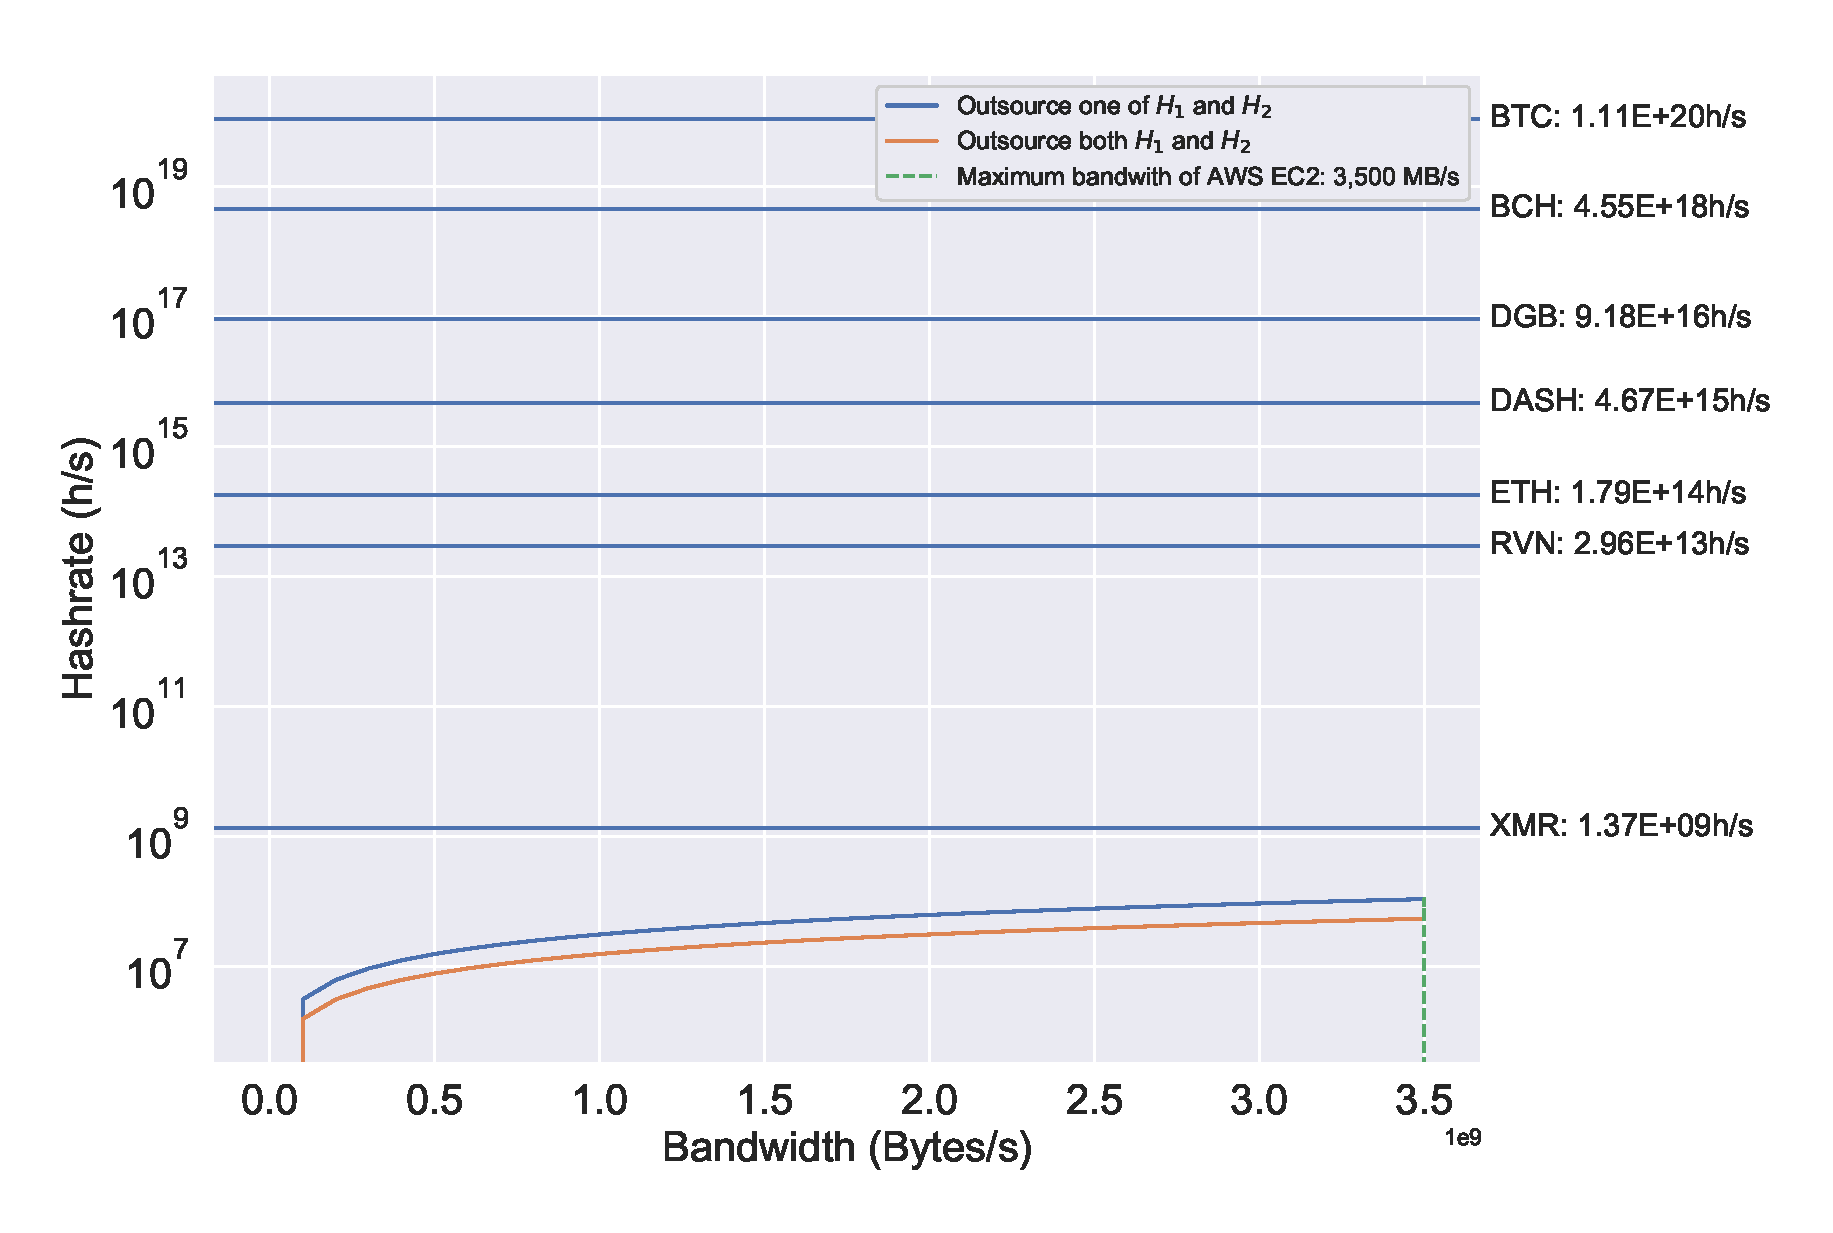
\includegraphics[width=.8\linewidth]{figs/max-hashrate.eps}
    \caption{Server bandwidth v.s. maximum hashrate. Data of server bandwidth and hashrate were fetched from AWS~\cite{aws} and CoinWarz~\cite{coinwarz}at 01/03/2020, respectively.}
    \label{fig:max-hashrate}
\end{figure}

Figure~\ref{fig:max-hashrate} shows relationship between the server's network bandwidth and the maximum hashrate the server can achieve.
The result shows that, existing servers can only achieve limited hashrate on partial outsourcing.
On AWS~\cite{aws}, I3EN Metal is the server with most bandwidth, which is 3,500 MB/s.
However, I3EN Metal can support hashrate less than $\frac{1}{10}$ of Monero's total mining power.
Within those mainstream cryptocurrencies, Monero's hashrate is the least.
Even if the pool operator rents a cluster of I3EN Metal machines for more bandwidth, I3EN Metal is quite expensive (10.848 USD per hour), leading to high expense of maintaining a mining pool.
Therefore, partial outsourcing in VRF-based mining is costly and unrealistic.








% \begin{figure}[]
%     \centering
%     \begin{msc}{}
%         \setlength{\envinstdist}{2.5cm}

%         \setlength{\instdist}{4cm}
%         \setlength{\instwidth}{1.5cm}
        
%         \declinst{pool}{}{Pool}
%         \declinst{miner}{}{Miner}

%         \action*{\parbox{4.5cm}{
%             Get block template $t$\\
%             Get pool mining difficulty $PT$\\
%             Get nonce interval $[n_1, n_m]$
%         }}{pool}

%         \nextlevel[4]
%         \mess{$n_1, n_m, t$}{pool}{miner}

%         \nextlevel
%         \action*{\parbox{3cm}{
%             For all $k \in [1, m]$\\
%             \tab $h_k \gets H_1(t||n_k)$
%         }}{miner}

%         \nextlevel[3]
%         \mess{$h_1, h_2, \dots, h_m$}{miner}{pool}

%         \nextlevel
%         \action*{\parbox{3.8cm}{
%             For all $k \in [1, m]$\\
%             \tab Check if $h_k = H(t||n_k)$\\
%             \tab $\gamma_k \gets {h_k}^{sk}$
%         }}{pool}

%         \nextlevel[5]
%         \mess{$\gamma_1, \gamma_2, \dots, \gamma_m, PT$}{pool}{miner}

%         \nextlevel
%         \action*{\parbox{3.5cm}{
%             $\Gamma \gets []$\\
%             For all $k \in [1, m]$\\
%             \tab $out_k \gets H_2(\gamma_k)$\\
%             \tab if $out_k < PT$\\
%             \tab\tab Append $\gamma_k$ to $\Gamma$
%         }}{miner}

%         \nextlevel[6]
%         \mess{$\Gamma$}{miner}{pool}

%         \nextlevel
%         \action*{\parbox{4.5cm}{
%             (Optional) For all $\gamma_j \in \Gamma$\\
%             \tab Check if $\gamma_j \in (\gamma_1, \dots, \gamma_m)$\\
%             \tab if $H_2(\gamma_j) < PT$\\
%             \tab\tab Mined a share 
%         }}{pool}

%         \nextlevel[5]

%     \end{msc}
%     \caption{Partial outsourcing in VRF-based mining.}
%     \label{fig:outsource-vrf}
% \end{figure}
